% SkillRC manuscript (ACL style, non-anonymous preprint layout).
% Build: bash build.sh   (pdflatex -> bibtex -> pdflatex x2)
\documentclass[11pt]{article}
\usepackage[preprint]{acl}

\usepackage{times}
\usepackage{latexsym}
\usepackage[T1]{fontenc}
\usepackage[utf8]{inputenc}
\usepackage{microtype}
\usepackage{inconsolata}
\usepackage{graphicx}
\usepackage{amsmath,amssymb}
\usepackage{booktabs}
\usepackage{multirow}
\usepackage{array}
\usepackage{enumitem}
\usepackage{tikz}
\usetikzlibrary{arrows.meta}
\usepackage{listings}

\definecolor{phaseA}{HTML}{6F9AD3}
\definecolor{phaseB}{HTML}{B07A8F}
\definecolor{phaseC}{HTML}{6E9F72}
\definecolor{salmon}{HTML}{D9735A}
\definecolor{gptblue}{HTML}{5F86C2}
\definecolor{qwenmint}{HTML}{4FA58C}
\lstnewenvironment{promptbox}[1]
  {\endgraf\smallskip\noindent{\small\bfseries #1}\endgraf\nopagebreak
   \lstset{basicstyle=\ttfamily\scriptsize, breaklines=true, breakatwhitespace=true,
     columns=fullflexible, keepspaces=true, showstringspaces=false, upquote=true,
     frame=leftline, rulecolor=\color{black!30}, xleftmargin=4pt, framexleftmargin=2pt}}
  {\smallskip}

\newcommand{\ci}[2]{$[#1,\,#2]$}
\newcolumntype{L}[1]{>{\raggedright\arraybackslash}p{#1}}

% let full-width floats share a page in the appendix
\renewcommand{\dbltopfraction}{0.95}
\renewcommand{\dblfloatpagefraction}{0.8}
\setcounter{dbltopnumber}{4}

\title{SkillRC: Is It the Skill or the Stack?\\Auditing Experience Memory in Agent Harnesses}

\author{Yiwen Lu \\
  University of Notre Dame \\
  \texttt{ylu37@nd.edu} \\[2pt]
  {\small Manuscript, 2026. Code and data: \url{https://github.com/EvenEureka/SkillRC}}}

\hypersetup{pdftitle={SkillRC: Is It the Skill or the Stack? Auditing Experience Memory in Agent Harnesses},
  pdfauthor={Yiwen Lu}}

\begin{document}
\maketitle

\begin{abstract}
Rules distilled from an agent's past runs can help one model and not another. Is the difference in
what the rules say, the skill, or in how each model reads added text, the stack? A control that keeps a
memory's items, tags, word counts, order and token count but replaces each rule with a sentence about
gardening splits the effect into reading cost and content value. The differences we could attribute lie
in the skill. On ALFWorld, no model's reading cost was distinguishable from zero, and all were within 0.04. The content was worth $+0.08$ to GPT-4o-mini on a pool from its own runs, $+0.039$ (95\% interval
\ci{0.012}{0.065}) to Qwen3-8B across 18 pools, and nothing measurable to the other four models. On
WebShop it lowered the scores of the two readers able to do the task. For Qwen3 readers, rules distilled
from experience beat equally long rules written without it by $+0.035$ \ci{0.014}{0.057}, and the source
agent made no difference at balanced coverage. Because only a matched control places an effect in the content, and pools built alike differ about as
much as these effects, a memory should be judged against a length-matched control over several pools.
\end{abstract}

\section{Introduction}
\label{sec:intro}

A common way to let an LLM agent learn from experience is to collect its successful runs, ask a language
model to distill them into a short list of rules, and place the list in the agent's prompt
\citep{zhao2023expel,shinn2023reflexion,wang2025awm}. The gains are uneven. Evaluations of agent skills
find gains that vary across tasks and models and are sometimes negative
\citep{li2026skillsbench,han2026sweskills}, and that shrink when skills have to be retrieved under
realistic conditions \citep{liu2026wildskills}. In our own runs, the same 33 rules raise GPT-4o-mini's
success on ALFWorld by 0.08 and change the success of Llama-3.1-8B, GPT-4.1-mini and Qwen3-14B by less
than 0.03. A practitioner cannot tell from such a result whether to change the rules or the model.

A comparison with and without the memory cannot settle this, because adding a memory changes two things
at once. The model has more text to read, and the text says something about the task. Language models
are sensitive to irrelevant context and to the length and format of their input
\citep{shi2023distracted,levy2024sametask,sclar2023quantifying}, so the first change alone could move
success by as much as the gains being reported. We call the effect of the first change the
\emph{reading cost} of a memory and the effect of the second its \emph{content value}. Our title asks
which of the two differs from one model to the next: the skill, meaning what the memory says, or the
stack, meaning the reader model with its tokenizer, chat template and serving. The harness, the layer
around the model that builds its context, exposes tools and retrieval, keeps memory and parses outputs
\citep{huang2026memoharness,lee2026metaharness}, is held fixed except for the memory block.

We call our evaluation design SkillRC, a reality check for agent skills. It measures the two parts with
a control that keeps everything about the memory except its content. The control has the same number of
items with the same tags, each item has the same number of words, the items appear in the same order,
and the block has the same token count under every reader's tokenizer, but each rule is replaced by a
sentence about vegetable gardening. The control minus no memory is the reading cost, and the memory minus
the control is the content value. Two further contrasts ask what the content value consists of. A list of
generic rules of the same length, written by a model that saw only a description of the task, tests
whether the value needs experience at all. A crossover of the agents that supply the experience with the
models that distill it, with three replicate pools for each pairing, tests whether it matters whose
experience it is and how much pools built the same way differ.

We find that no reader pays a measurable cost for reading a memory-length block, and that the reader
differences we could attribute lie in what the memory says. The content was worth $+0.08$ to
GPT-4o-mini, reading a pool built from its own runs, about $+0.04$ to Qwen3-8B across 18 pools, nothing
measurable to the other four readers on ALFWorld, and a loss on WebShop for both readers that can do the
task. For the Qwen3 readers we tested, distilled rules beat generic rules of the same length, and the
agent that supplied the experience made no difference once coverage was equal. Two pools built by the
same pipeline can differ by as much as these effects.

Our contribution is an evaluation design for experience memory: a decomposition into reading cost and
content value with controls matched in items, order and token count, and audits that check that every
task receives the same items in the same order under each condition (\S\ref{sec:method}). We apply it in
five studies on ALFWorld \citep{shridhar2021alfworld} and WebShop \citep{yao2022webshop} whose
predictions were written down before their runs (\S\ref{sec:results}), with six readers and 24 ALFWorld
pools in all.

\section{Related Work}
\label{sec:related}

Agents that learn from experience store it in many forms: executable skills \citep{wang2024voyager},
verbal reflections \citep{shinn2023reflexion}, distilled insights and guidelines
\citep{zhao2023expel,fu2024autoguide}, reusable workflows \citep{wang2025awm}, evolving playbooks
\citep{zhang2026ace}, and strategies distilled from both successes and failures
\citep{ouyang2026reasoningbank}. Later systems curate or revise skills around a fixed executor
\citep{yang2026skillopt,ouyang2026skillos,gao2026selfevoskill}, or optimize the whole harness in which
a memory sits \citep{lee2026metaharness,huang2026memoharness}. Most of this work supports its methods
with a gain over the same agent without memory, usually measured on one or two strong models.

Evaluations that look across tasks and models find such gains unstable. SkillsBench reports broad
average gains from curated skills together with negative deltas on some tasks, and it notes that an
injected skill also adds context, using self-generated skills as a partial control
\citep{li2026skillsbench}. SWE-Skills-Bench finds limited gains and a token overhead in software
engineering \citep{han2026sweskills}, and realistic retrieval erodes skill gains further
\citep{liu2026wildskills}. On ALFWorld, abstract procedural memories transfer better than raw
trajectories, with negative transfer concentrated on hard cases \citep{hu2026memory}, and agents follow
retrieved experience closely enough to be misled by it \citep{xiong2026memory}. SelfEvoSkill compares
executions with and without a skill while holding the agent, task and workspace fixed, and uses the
difference to revise the skill \citep{gao2026selfevoskill}; we use the same kind of matched comparison
to evaluate a fixed memory, adding a control for the act of reading. These studies show that the effect
of a memory varies, without separating the part due to reading added text.

Prompting research has made that kind of separation for a long time. Content-free inputs calibrate
few-shot predictions \citep{zhao2021calibrate}, irrelevant or misleading instructions can work about as
well as good ones \citep{webson2022prompt}, and demonstrations with random labels keep much of their
benefit \citep{min2022rethinking}. Irrelevant context, longer inputs, formatting and position all change
what a model does \citep{shi2023distracted,levy2024sametask,sclar2023quantifying,liu2024lost}. On
ALFWorld itself, ReAct performance is driven by the similarity between demonstration tasks and queries
more than by the content of the reasoning traces \citep{verma2024brittle}. Most of these controls were
designed for a single prompt. An agent's memory is reread at every step of an episode, by
models whose tokenizers and handling of context differ, and its content is distilled from experience
that might be replaceable by advice requiring none. We have not found a study that separates reading
cost from content value for agent memory across readers, asks whether the content value is specific to
experience, or measures how much it changes between pools built by the same pipeline. These are the
questions we take up.

\section{Method}
\label{sec:method}

\begin{figure*}[t]
\centering
% SkillRC design schematic (TikZ), included by manuscript_body.tex. Plots no data.
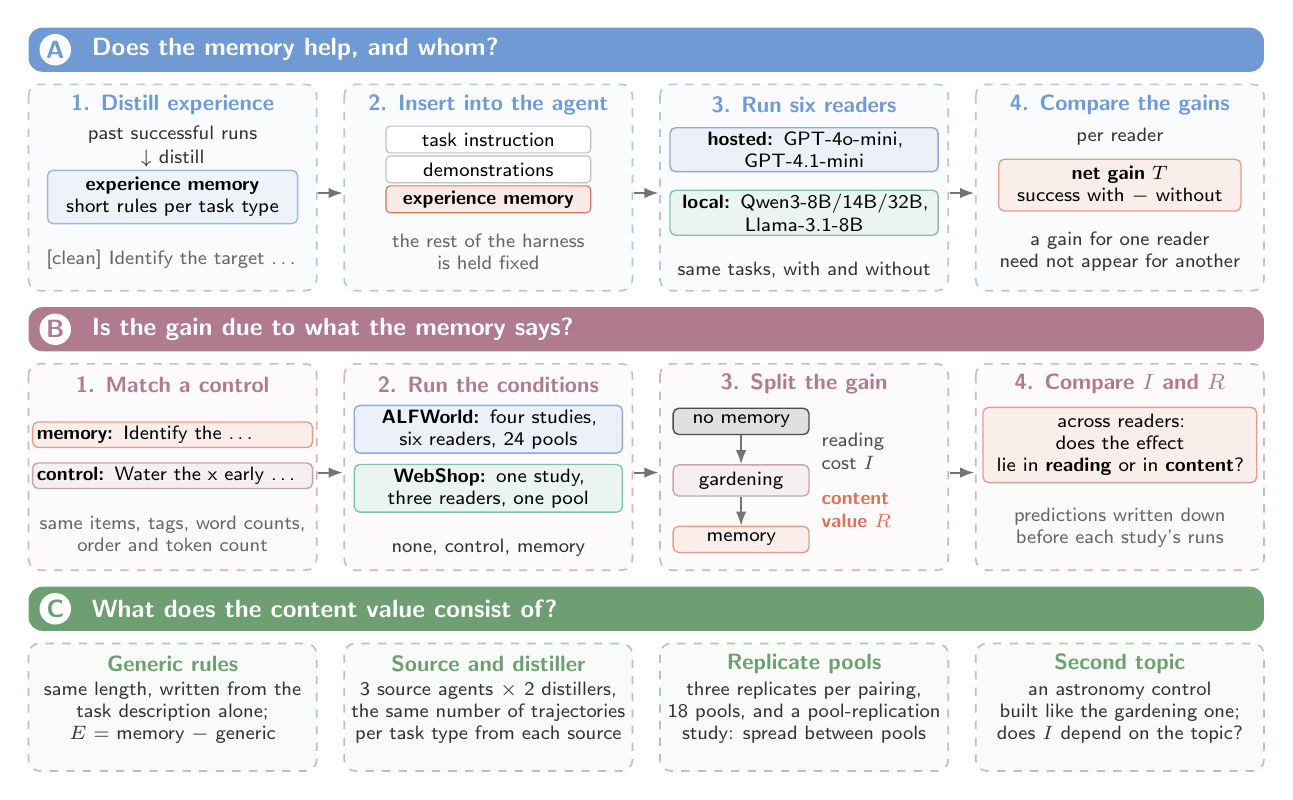
\begin{tikzpicture}[
  x=1cm, y=1cm,
  font=\sffamily\scriptsize,
  col/.style={draw=#1!55, dashed, rounded corners=4pt, fill=#1!4, line width=0.6pt},
  steptitle/.style={font=\sffamily\bfseries\footnotesize, text=#1},
  body/.style={align=center, text=black!80, font=\sffamily\scriptsize},
  note/.style={align=center, text=black!60, font=\sffamily\scriptsize},
  card/.style={draw=#1!70, fill=#1!12, rounded corners=2pt, line width=0.5pt, align=center,
               font=\sffamily\scriptsize, inner sep=2.5pt},
  flow/.style={-{Latex[length=1.8mm]}, draw=black!55, line width=0.7pt},
  layer/.style={draw=black!25, fill=white, rounded corners=1.5pt, minimum width=2.6cm,
                minimum height=0.34cm, font=\sffamily\scriptsize, inner sep=1pt},
]
\def\cw{3.66}\def\gap{0.35}
\pgfmathsetmacro{\step}{\cw+\gap}
\pgfmathsetmacro{\W}{4*\cw+3*\gap}
\pgfmathsetmacro{\hc}{\cw/2}

% ============================ Band A =======================================
\fill[phaseA, rounded corners=5pt] (0,0) rectangle (\W,-0.56);
\fill[white] (0.34,-0.28) circle (0.2);
\node[font=\sffamily\bfseries\small, text=phaseA] at (0.34,-0.28) {A};
\node[anchor=west, font=\sffamily\bfseries\small, text=white] at (0.68,-0.28)
  {Does the memory help, and whom?};
\foreach \i in {0,...,3} { \draw[col=phaseA] (\i*\step,-0.72) rectangle ++(\cw,-2.62); }

\node[steptitle=phaseA] at (\hc,-0.98) {1. Distill experience};
\node[body] at (\hc,-1.36) {past successful runs};
\node[body] at (\hc,-1.66) {$\downarrow$ distill};
\node[card=phaseA, text width=3.0cm] at (\hc,-2.15) {\textbf{experience memory}\\short rules per task type};
\node[note] at (\hc,-2.95) {[clean] Identify the target \ldots};

\node[steptitle=phaseA] at (\hc+\step,-0.98) {2. Insert into the agent};
\node[layer] at (\hc+\step,-1.42) {task instruction};
\node[layer] at (\hc+\step,-1.80) {demonstrations};
\node[layer, draw=salmon, fill=salmon!15, font=\sffamily\bfseries\scriptsize] at (\hc+\step,-2.18) {experience memory};
\node[note] at (\hc+\step,-2.85) {the rest of the harness\\is held fixed};

\node[steptitle=phaseA] at (\hc+2*\step,-0.98) {3. Run six readers};
\node[card=gptblue, text width=3.3cm, inner sep=1.5pt] at (\hc+2*\step,-1.55) {\textbf{hosted:} GPT-4o-mini,\\GPT-4.1-mini};
\node[card=qwenmint, text width=3.3cm, inner sep=1.5pt] at (\hc+2*\step,-2.35) {\textbf{local:} Qwen3-8B/14B/32B,\\Llama-3.1-8B};
\node[body] at (\hc+2*\step,-3.08) {same tasks, with and without};

\node[steptitle=phaseA] at (\hc+3*\step,-0.98) {4. Compare the gains};
\node[body] at (\hc+3*\step,-1.38) {per reader};
\node[card=salmon, text width=2.9cm] at (\hc+3*\step,-2.0) {\textbf{net gain} $T$\\success with $-$ without};
\node[body] at (\hc+3*\step,-2.85) {a gain for one reader\\need not appear for another};

\foreach \i in {0,...,2} { \draw[flow] (\i*\step+\cw+0.02,-2.1) -- (\i*\step+\cw+\gap-0.02,-2.1); }

% ============================ Band B =======================================
\def\yb{-3.55}
\fill[phaseB, rounded corners=5pt] (0,\yb) rectangle (\W,\yb-0.56);
\fill[white] (0.34,\yb-0.28) circle (0.2);
\node[font=\sffamily\bfseries\small, text=phaseB] at (0.34,\yb-0.28) {B};
\node[anchor=west, font=\sffamily\bfseries\small, text=white] at (0.68,\yb-0.28)
  {Is the gain due to what the memory says?};
\foreach \i in {0,...,3} { \draw[col=phaseB] (\i*\step,\yb-0.72) rectangle ++(\cw,-2.62); }

\node[steptitle=phaseB] at (\hc,\yb-0.98) {1. Match a control};
\node[card=salmon, text width=3.45cm, align=left, inner sep=1.5pt] at (\hc,\yb-1.62)
  {\textbf{memory:} Identify the \ldots};
\node[card=phaseB, text width=3.45cm, align=left, inner sep=1.5pt] at (\hc,\yb-2.14)
  {\textbf{control:} Water the x early \ldots};
\node[note] at (\hc,\yb-2.88) {same items, tags, word counts,\\order and token count};

\node[steptitle=phaseB] at (\hc+\step,\yb-0.98) {2. Run the conditions};
\node[card=gptblue, text width=3.3cm, inner sep=1.5pt] at (\hc+\step,\yb-1.55) {\textbf{ALFWorld:} four studies,\\six readers, 24 pools};
\node[card=qwenmint, text width=3.3cm, inner sep=1.5pt] at (\hc+\step,\yb-2.3) {\textbf{WebShop:} one study,\\three readers, one pool};
\node[body] at (\hc+\step,\yb-3.05) {none, control, memory};

\node[steptitle=phaseB] at (\hc+2*\step,\yb-0.98) {3. Split the gain};
\node[card=black, text width=1.55cm] (n0) at (\hc+2*\step-0.8,\yb-1.45) {no memory};
\node[card=phaseB, text width=1.55cm] (n1) at (\hc+2*\step-0.8,\yb-2.2) {gardening};
\node[card=salmon, text width=1.55cm] (n2) at (\hc+2*\step-0.8,\yb-2.95) {memory};
\draw[flow] (n0.south) -- (n1.north);
\draw[flow] (n1.south) -- (n2.north);
\node[font=\sffamily\scriptsize, text=black!70, anchor=west, align=left] at (\hc+2*\step+0.1,\yb-1.83) {reading\\cost $I$};
\node[font=\sffamily\scriptsize\bfseries, text=salmon, anchor=west, align=left] at (\hc+2*\step+0.1,\yb-2.58) {content\\value $R$};

\node[steptitle=phaseB] at (\hc+3*\step,\yb-0.98) {4. Compare $I$ and $R$};
\node[card=salmon, text width=3.3cm] at (\hc+3*\step,\yb-1.75) {across readers: does the effect\\lie in \textbf{reading} or in \textbf{content}?};
\node[note] at (\hc+3*\step,\yb-2.8) {predictions written down\\before each study's runs};

\foreach \i in {0,...,2} { \draw[flow] (\i*\step+\cw+0.02,\yb-2.1) -- (\i*\step+\cw+\gap-0.02,\yb-2.1); }

% ============================ Band C =======================================
\def\yc{-7.1}
\fill[phaseC, rounded corners=5pt] (0,\yc) rectangle (\W,\yc-0.56);
\fill[white] (0.34,\yc-0.28) circle (0.2);
\node[font=\sffamily\bfseries\small, text=phaseC] at (0.34,\yc-0.28) {C};
\node[anchor=west, font=\sffamily\bfseries\small, text=white] at (0.68,\yc-0.28)
  {What does the content value consist of?};
\foreach \i in {0,...,3} { \draw[col=phaseC] (\i*\step,\yc-0.72) rectangle ++(\cw,-1.62); }

\node[steptitle=phaseC] at (\hc,\yc-0.98) {Generic rules};
\node[body] at (\hc,\yc-1.6) {same length, written from the\\task description alone;\\$E$ = memory $-$ generic};

\node[steptitle=phaseC] at (\hc+\step,\yc-0.98) {Source and distiller};
\node[body] at (\hc+\step,\yc-1.6) {3 source agents $\times$ 2 distillers,\\the same number of trajectories\\per task type from each source};

\node[steptitle=phaseC] at (\hc+2*\step,\yc-0.98) {Replicate pools};
\node[body] at (\hc+2*\step,\yc-1.6) {three replicates per pairing,\\18 pools, and a pool-replication\\study: spread between pools};

\node[steptitle=phaseC] at (\hc+3*\step,\yc-0.98) {Second topic};
\node[body] at (\hc+3*\step,\yc-1.6) {an astronomy control\\built like the gardening one;\\does $I$ depend on the topic?};
\end{tikzpicture}

\caption{The design. A memory distilled from past runs is inserted as one block into an otherwise fixed
agent and read by six models (A). A matched control with the same items, order and token count splits
each reader's gain into a reading cost and a content value (B). Further contrasts ask what the content
value consists of (C).}
\label{fig:design}
\end{figure*}

\subsection{Reading cost and content value}
\label{sec:decomposition}

An experience memory here is a pool of short rules, each tagged with a task type, distilled from
successful trajectories and inserted as one block into the prompt of a frozen model, the
\emph{reader}. The harness ranks the items against the current task with BM25
\citep{robertson2009bm25} and inserts them up to a token budget. In all our studies the whole pool fits,
so ranking only sets the order. Nothing else in the prompt changes (Figure~\ref{fig:design}). For each
task $t$, the realized payload of a condition is the set of pool positions it inserts, $I_t$, their order
$\sigma_t$ and their token count $\ell_t$. Two conditions are \emph{payload-matched} when $I_t$ and
$\sigma_t$ coincide for every task and $\ell_t$ is equal under every reader's tokenizer. The harness logs
$\ell_t$ in every episode, and an offline audit replays the retrieval on every task to check $I_t$ and
$\sigma_t$.

Let $\bar Y_{\text{none}}$, $\bar Y_{\text{mem}}$ and $\bar Y_{\text{irr}}$ be a reader's mean success
without memory, with the memory and with the irrelevant control. The net effect splits as
\begin{equation}
\label{eq:decomp}
\underbrace{\bar Y_{\text{mem}}-\bar Y_{\text{none}}}_{T\text{, net effect}}
=\underbrace{\bar Y_{\text{irr}}-\bar Y_{\text{none}}}_{I\text{, reading cost}}
+\underbrace{\bar Y_{\text{mem}}-\bar Y_{\text{irr}}}_{R\text{, content value}} .
\end{equation}
A reading cost can be positive if an added block of any content helps. The split assumes that the cost
of reading does not depend on what the text is about, an assumption we return to in
Section~\ref{sec:what}. It is also only as good as the control, which is payload-matched to the memory and, as far
as we could check, differs from it only in content. Each item keeps its tag and its word count, and its
body becomes an imperative sentence about vegetable gardening, drawn from a bank of templates that use no
ALFWorld object, receptacle or action word (Table~\ref{tab:examples}). We wanted the control to read like
advice. It is ranked with the true pool's BM25 scores and inserted at the same positions. A deterministic
pass then replaces the fewest body words with the nonce token \texttt{x} until the block has the memory's
token count under the tokenizer of every reader in the study. The 18 crossover controls and the astronomy
controls needed no replacement. The focal pool's control, used in the five-reader and generic-rule
studies, needed 30 replacements in 472 body words, spread over 19 of its 33 items (for example ``Rotate
crops every x x then x x then x to rest the tired soil''). The Qwen-sourced pool's control and one
pool-replication control needed 3 each, and the WebShop control, about choral singing because WebShop
sells garden products, needed 20 in 377 body words.

\begin{table}[t]
\centering
\small
\setlength{\tabcolsep}{4pt}
\renewcommand{\arraystretch}{1.12}
\begin{tabular}{@{}lL{0.74\columnwidth}@{}}
\toprule
Condition & Item 3 of the focal pool, tag \texttt{[clean]} \\
\midrule
Memory & Always clean the item using the designated cleaning area before placing it in the final location. \\
Generic & To verify the task is complete, carefully examine the object or look at the receptacle closely. \\
Gardening & Always pull weeds while they are small so they never set seed across the whole garden. \\
Astronomy & Mount the camera on a sturdy tracking head and begin with short exposures of bright constellations. \\
\bottomrule
\end{tabular}
\caption{One item in each condition, copied from the released pools. All four have 16 words, and each
whole block has the memory's token count under every reader's tokenizer. This gardening item needed no
placeholder.}
\label{tab:examples}
\end{table}

All estimates in this paper are differences of paired task means. Intervals are 95\% percentile
intervals from 20,000 bootstrap draws of tasks within task type (product category on WebShop), with
pools also resampled where Section~\ref{sec:crossover} says so.

\subsection{What the content value consists of}
\label{sec:crossover}

\paragraph{Experience or generic advice.} If the distilled rules only restated what a model can infer
from the task description, a list written without any experience should do as well. For each ALFWorld
task type, Qwen3-32B received a fixed description of the environment and of the goal, together with the
instruction wording of the distillation prompt, and wrote six rules without seeing a trajectory. The
rules were then paired with the memory's items, rewritten to the same word count and matched in token
count and order (Appendix~\ref{app:controls}). The contrast
$E=\bar Y_{\text{mem}}-\bar Y_{\text{gen}}$ is what experience adds beyond generic advice, and
$G=\bar Y_{\text{gen}}-\bar Y_{\text{irr}}$ is what generic advice adds over unrelated text. A second
unrelated control about amateur astronomy, built like the gardening one, shows how much the reading
cost depends on the topic of the control.

\paragraph{Source, distiller and replicate pools.} Pools distilled from different agents differ in
coverage as well as in whose experience they hold. On the 140 seen ALFWorld games, GPT-4o-mini succeeded
in 73 games, Qwen3-8B in 111 and Qwen3-32B in 116, and GPT-4o-mini solved only one heat game. A pool
built from all successes therefore confounds the source with how much of the task its trajectories
cover. We drew the same number of successful trajectories per task type from each source, six per type
except one for heat, 31 in all. Each source has three replicate subsamples drawn with different seeds,
and each subsample was distilled once by Qwen3-32B and once by Qwen3-8B with the same prompt. The result
is 18 pools of 31 to 36 rules (660 to 777 tokens), each with its own gardening control. Intervals for
pooled estimates resample tasks within type and, for each source, its three subsamples, so they include
the variation between pools. A smaller pool-replication study took the same approach with one source,
one distiller and one reader: Qwen3-32B distilled four pools from Qwen3-8B's successes, the first six
trajectories per type and three random subsamples of six per type, and Qwen3-8B read them.

\subsection{Readers, environments and studies}
\label{sec:setup}

\paragraph{ALFWorld.} We use the 134 unseen games with a ReAct scaffold \citep{yao2023react} that lists
the admissible actions, two demonstrations per prompt and a limit of 30 steps. Each run covers every
game with three demonstration pairs, 402 episodes. The focal pool holds 33 rules (645 tokens) that
GPT-4o-mini distilled from at most six of its own successful trajectories per task type on the seen
games. The generic-rule and pool-replication studies also use a second pool, which we call the
Qwen-sourced pool: 36 rules (706 tokens) that GPT-4o-mini distilled from Qwen3-8B's successes.

\paragraph{WebShop.} WebShop replaces rooms and objects with search and product pages, so it tests whether
the decomposition carries over to a different action space. We use the 1,000-product environment with a server that seeds its random
generation of prices, so that every session has the same instruction across restarts. The 500 test
sessions allow 15 steps and are scored in $[0,1]$. The pool holds 30 rules (524 tokens) that
GPT-4o-mini distilled from its own successes on 576 training sessions.

\paragraph{Readers.} Our question concerns differences between readers, so the readers span a range of
ability, from 0.26 to 0.90 success without memory on ALFWorld. GPT-4o-mini and GPT-4.1-mini are called
through the OpenAI API. Llama-3.1-8B
\citep{grattafiori2024llama3} and Qwen3-8B, Qwen3-14B and Qwen3-32B \citep{yang2025qwen3}, with
thinking off, are served locally with vLLM \citep{kwon2023vllm}. All decode at temperature zero.
Table~\ref{tab:studies} lists the five studies.

\begin{table*}[t]
\centering
\small
\setlength{\tabcolsep}{5pt}
\renewcommand{\arraystretch}{1.12}
\begin{tabular}{@{}llL{0.29\textwidth}L{0.19\textwidth}L{0.20\textwidth}@{}}
\toprule
Study & Environment & Readers & Memories & Conditions \\
\midrule
Five readers & ALFWorld & GPT-4o-mini, GPT-4.1-mini, Llama-3.1-8B, Qwen3-8B, Qwen3-14B & focal pool & none, memory, gardening \\
WebShop & WebShop & GPT-4o-mini, GPT-4.1-mini, Qwen3-8B & one pool & none, memory, choral singing \\
Crossover & ALFWorld & Qwen3-8B, Qwen3-14B, Qwen3-32B & 18 balanced pools & none, memory, gardening \\
Generic rules & ALFWorld & Qwen3-8B, Qwen3-14B & focal and Qwen-sourced pools & the above, generic rules, astronomy \\
Pool replication & ALFWorld & Qwen3-8B & four replicate pools and the Qwen-sourced pool & none, memory, gardening \\
\bottomrule
\end{tabular}
\caption{The five studies. Every condition of a study ran for each of its readers in one time window,
with 402 episodes per ALFWorld run and 500 sessions per WebShop run. GPT-4o-mini ran every condition of
the first two studies twice.}
\label{tab:studies}
\end{table*}

\paragraph{Protocols and noise.} For each study we wrote down the predictions, estimands and analysis
before its runs. In the five-reader study, one addendum (D1--D2) was written after the hosted readers'
runs had been analysed (Appendix~\ref{app:protocols}). We call these protocol analyses and mark everything
chosen after seeing data as exploratory. Appendix~\ref{app:protocols} lists every prediction with its
outcome. The first two studies also included a scrambled copy of the memory, with each item's words
shuffled until no original adjacent pair remained, as a second control. Its effect changed sign between
game samples for the same reader, so we report only the gardening control. Repeating a run under
identical settings changes the outcome of 17--20\% of GPT-4o-mini episodes and 4--13\% of local-reader
episodes, so we read differences of about 0.02 between single runs as noise.

\section{Results}
\label{sec:results}

\begin{figure*}[t]
\centering
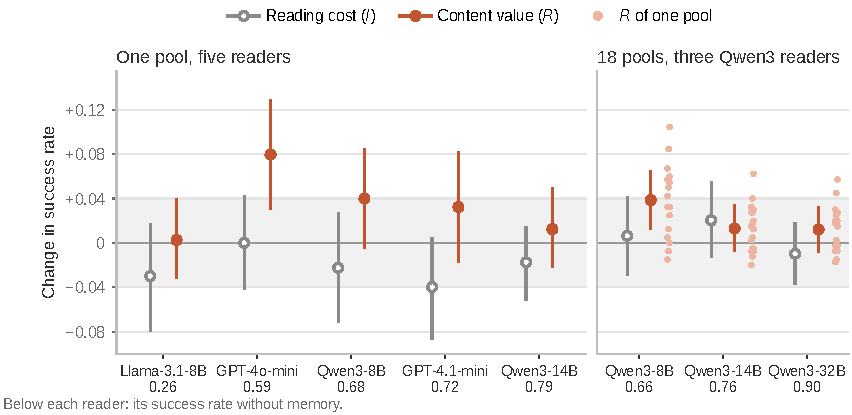
\includegraphics[width=\textwidth]{figures/fig_readers.pdf}
\caption{Reading cost $I$ (unrelated text minus no memory) and content value $R$ (memory minus
unrelated text) on 134 unseen ALFWorld games, with 95\% intervals. Left: the focal pool read by five
readers (single runs). Right: the mean over 18 pools for three Qwen3 readers, with intervals that
resample pools as well as tasks. Light dots are the content values of the individual pools. The shaded
band marks $\pm0.04$, the bound predicted for the crossover.}
\label{fig:readers}
\end{figure*}

\subsection{No reader pays a measurable reading cost}
\label{sec:cost}

With the focal pool, the gardening control changes success by 0.000 for GPT-4o-mini and by $-0.017$ to
$-0.040$ for the other four readers, and every interval includes zero (Figure~\ref{fig:readers}, left).
We had expected the reading cost to explain why a memory helps some readers and not others, because a
memory adds several hundred tokens of instructions and models differ in how they handle added context.
In an addendum written before the local readers' estimates were computed, the five-reader study
therefore predicted that the reading cost would vary across readers more than the content value. That
prediction failed. Across the five readers the reading cost spans 0.040 and the content value 0.077.
The difference between the two spans is itself uncertain, \ci{-0.050}{0.095} (exploratory), and so are
the differences between readers' reading costs, whose intervals reach 0.10. For GPT-4.1-mini minus
GPT-4o-mini, for instance, the difference is $-0.040$ \ci{-0.100}{0.020}.

The $\pm0.04$ band was set from the range of these five estimates and then used as a prediction for the
crossover, so for the five readers above it is a description, not a test. The intervals rule out reading
costs beyond $\pm0.04$ only for GPT-4o-mini averaged over its two runs, \ci{-0.037}{0.031}, and for
Qwen3-32B. In the crossover, averaged over pools, the reading cost is $+0.006$ for Qwen3-8B, $+0.020$ for
Qwen3-14B and $-0.010$ for Qwen3-32B, inside the predicted band, and no single pool's control moves any of
the three readers by more than 0.037. Across all studies the largest single-pool estimate is $-0.042$.
On WebShop the choral control changes the score by $+0.018$ for GPT-4o-mini and $-0.016$ for Qwen3-8B
(Table~\ref{tab:webshop}).

The topic of the unrelated text matters more than we expected. The generic-rule study predicted that
replacing gardening with amateur astronomy would shift the reading cost by less than 0.03, with an
interval including zero. The shift was 0.025 \ci{0.007}{0.044}, small but distinguishable from zero, so
the reading cost is $+0.017$ \ci{-0.010}{0.045} under one topic and $-0.007$ \ci{-0.034}{0.019} under the
other. Measured against the astronomy control, Qwen3-8B's content value in that study would be about
$+0.075$ instead of $+0.044$ (exploratory), and absolute content values carry a margin of this size.

\subsection{Two readers gain reliably from the content}
\label{sec:reader}

Content value is reliably positive for two readers, GPT-4o-mini with the focal pool and Qwen3-8B across
18 pools. With the focal pool, content values range from $+0.002$ to $+0.080$, and only GPT-4o-mini's
excludes zero, at $+0.080$ \ci{0.030}{0.129} in the protocol run and $+0.091$ \ci{0.050}{0.133} averaged
over its two runs. On the 74 games added after the first 60, it is $+0.059$ \ci{-0.009}{0.126}.
Qwen3-8B follows at $+0.040$, GPT-4.1-mini at $+0.032$, Qwen3-14B at $+0.012$ and Llama-3.1-8B at
$+0.002$. GPT-4o-mini's content value exceeds Llama-3.1-8B's by 0.077 \ci{0.012}{0.142} and Qwen3-14B's
by 0.067 \ci{0.012}{0.122}, unadjusted for multiplicity. Against GPT-4.1-mini, the gap in net effect,
0.087 \ci{0.025}{0.152}, splits about evenly between reading cost (0.040) and content value (0.047),
neither of them reliable on its own. GPT-4o-mini is also the agent whose trajectories, distilled by
GPT-4o-mini, make up the focal pool, so its lead may partly be an own-source advantage, which the
crossover could not resolve (\S\ref{sec:what}).

Over 18 pools (Figure~\ref{fig:readers}, right), the content value is $+0.039$ \ci{0.012}{0.065} for
Qwen3-8B, $+0.013$ \ci{-0.008}{0.034} for Qwen3-14B and $+0.012$ \ci{-0.008}{0.033} for Qwen3-32B. The
crossover's protocol predicted that Qwen3-8B would gain reliably more than Qwen3-32B. The difference,
$+0.026$ \ci{-0.007}{0.060}, does not meet that bar (Holm-adjusted $p=0.52$), so the ordering by size
remains a trend.

Exploratory: content value was reliable only for two mid-range readers, whose success without memory is
0.59 and 0.66--0.68; we note this pattern without testing it. Llama-3.1-8B solves a quarter of the games
without memory and gains nothing. If each GPT-4o-mini episode is classified by how it did on the same game
in the other two no-memory episodes, its content value is $+0.196$ where it failed both and $+0.006$ where
it solved both, a difference of $+0.190$ \ci{0.076}{0.309}. Llama-3.1-8B gains nothing even on the
games it fails.

\subsection{Distilled rules beat generic rules, and pools differ as much as the effects}
\label{sec:what}

\begin{figure*}[t]
\centering
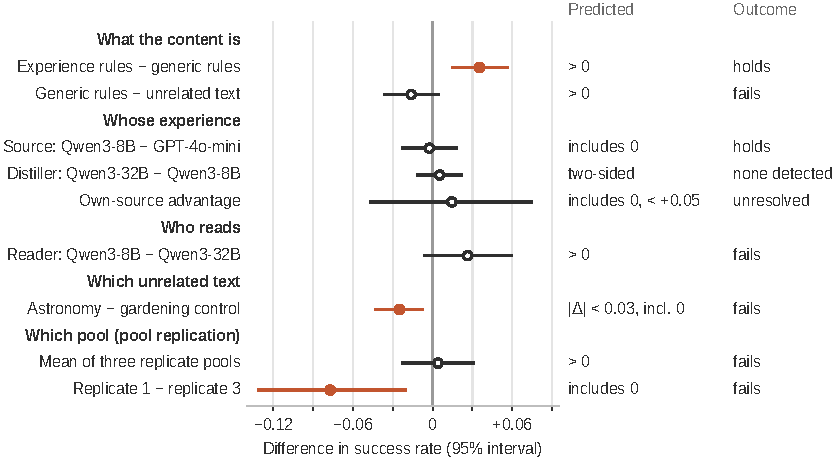
\includegraphics[width=\textwidth]{figures/fig_contrasts.pdf}
\caption{Protocol contrasts of the generic-rule study (pooled over two pools and two readers), the
crossover (pooled over pools and three readers) and the pool-replication study (reader Qwen3-8B), each
with its prediction and outcome. Filled markers have intervals that exclude zero.}
\label{fig:contrasts}
\end{figure*}

In the generic-rule study, read by Qwen3-8B and Qwen3-14B, experience rules beat generic rules of the
same length by $+0.035$ \ci{0.014}{0.057} over two pools and two readers, as predicted, with $+0.058$ for
Qwen3-8B and $+0.012$ for Qwen3-14B (Figure~\ref{fig:contrasts}). The study also predicted that the
generic rules would beat the gardening text, which they did not, at $-0.016$ \ci{-0.037}{0.005}. About
half of the gap is therefore the content value of the experience rules in this study, $+0.019$
\ci{-0.002}{0.040}, and the rest is the generic rules doing slightly worse than unrelated text. The gap
is not explained by greater word overlap with the test games: the generic rules share more words with
them than the distilled pools do, 8.5--9.3\% of their words against 3.9--5.5\%. The two lists also differ
in their writer. The experience pools were distilled by GPT-4o-mini and the generic rules written by
Qwen3-32B. On the focal pool, Qwen3-8B's advantage for experience comes entirely from generic rules doing
worse than gardening, $-0.062$ \ci{-0.104}{-0.020}. Text about the task may cost more to read than text
about gardening, in which case part of what we call content value is a reading cost that depends on
content.

The agent that supplied the experience made no difference once coverage was equal. With six
trajectories per type from each source (one for heat), the content value of pools built from Qwen3-8B's
successes and from GPT-4o-mini's differs by $-0.002$ \ci{-0.024}{0.019} for the three Qwen3
readers, as predicted, and Qwen3-32B's pools differ from Qwen3-8B's by $-0.006$ \ci{-0.029}{0.015}.
Qwen3-32B and Qwen3-8B distillations of the same subsamples differ by $+0.005$ \ci{-0.012}{0.022}, so
the distilling model made no detectable difference either. Whether a reader gains more from its own
experience is unresolved, at $+0.015$ \ci{-0.047}{0.075}. These results concern what a trajectory
contributes for Qwen3 readers. A more successful agent still leaves more trajectories, and the balanced
design removes that advantage by construction.

For a fixed source, distiller and reader, the crossover's three replicate pools differ by more than task
sampling explains ($Q=72.2$ on 36 degrees of freedom, $p=0.0003$). The between-pool standard deviation
of 0.019 is close to the 0.02 we had predicted and comparable to the content values themselves. For
Qwen3-8B, single pools range from $-0.015$ to $+0.105$. Two distillations of the same subsample agree
only moderately, with a correlation of 0.42 over 27 pairs, so both the choice of trajectories and the
distillation contribute. Single-pool content values should be read with this spread in mind, and the
pooled intervals in this section and in Figure~\ref{fig:readers} resample pools as well as tasks.

The pool-replication study points the same way (Table~\ref{tab:poolrep}). Its three random subsamples
gave Qwen3-8B content values of $-0.025$, $-0.015$ and $+0.052$, a mean of $+0.004$ \ci{-0.023}{0.032},
and the pool from the first six trajectories per type gave $+0.032$. The crossover pools with the same
source, distiller and reader gave $+0.041$ \ci{0.005}{0.077}, though they kept one heat trajectory where
these kept six. The study had predicted that its pools would carry value and agree with one another.
Both predictions failed: the first and third subsamples differ by $-0.077$ \ci{-0.132}{-0.020}.

\subsection{On WebShop the distilled rules lower both capable readers' scores}
\label{sec:webshop}

\begin{table}[!b]
\centering
\small
\setlength{\tabcolsep}{2.6pt}
\renewcommand{\arraystretch}{1.12}
\begin{tabular}{@{}lcccrr@{}}
\toprule
Reader & none & choral & memory & \multicolumn{1}{c}{$I$} & \multicolumn{1}{c}{$R$} \\
\midrule
GPT-4o-mini (1) & 0.294 & 0.312 & 0.154 & $+0.018$ & $-0.158$ \\
GPT-4o-mini (2) & 0.303 & 0.323 & 0.167 & $+0.020$ & $-0.156$ \\
Qwen3-8B & 0.329 & 0.313 & 0.198 & $-0.016$ & $-0.116$ \\
GPT-4.1-mini & 0.029 & 0.028 & 0.027 & $-0.001$ & $-0.002$ \\
\bottomrule
\end{tabular}
\caption{WebShop, 500 test sessions: mean score per condition, reading cost $I$ and content value $R$,
with GPT-4o-mini's two runs. Every $R$ interval for GPT-4o-mini and Qwen3-8B excludes zero and every $I$
interval includes it (Appendix~\ref{app:results}). GPT-4.1-mini fails almost every session in every
condition.}
\label{tab:webshop}
\end{table}

On WebShop the content value is negative (Table~\ref{tab:webshop}). The pool lowers GPT-4o-mini's score
from 0.294 to 0.154 while the choral control leaves it at 0.312, a content value of $-0.158$
\ci{-0.191}{-0.125}, and a second run gives $-0.156$. For Qwen3-8B it is $-0.116$ \ci{-0.153}{-0.079}.
The protocol had predicted a positive value for GPT-4o-mini. GPT-4.1-mini fails nearly every session in
every condition, so its estimates carry no information; in an exploratory reading of its sessions, it
typically opens one of a product's sub-pages, which have no Buy button, and keeps clicking there until
the step limit. In an exploratory count of actions, the pool raises GPT-4o-mini's searches per session
from 2.44 to 5.69, against 2.35 with the control, and Qwen3-8B's from 1.88 to 2.71. Several rules tell
the agent to search again, such as ``If the desired product is not found, consider re-searching with
the same criteria'' for fashion, the category of most test sessions. GPT-4o-mini, the reader with the
largest content value on ALFWorld, has the largest loss here, and its reading cost is near zero in both
environments.

\section{Conclusion}
\label{sec:conclusion}

The differences between models that we could attribute lie in the skill, in what the memory says.
Reading a memory of 520 to 790 tokens cost no model we tested a measurable amount, while what the rules
said was worth $+0.08$ to GPT-4o-mini on a pool from its own runs, about $+0.04$ to Qwen3-8B, nothing
measurable to the other four readers on ALFWorld, and a loss on WebShop.

Where a memory did nothing for a model, as for Llama-3.1-8B and Qwen3-14B with the focal pool and
Qwen3-32B across 18 pools, its content value was near zero and so was its reading cost, so no cost of
reading was masking a gain. GPT-4o-mini's lead over Llama-3.1-8B and Qwen3-14B lies in content value,
with no detectable difference in reading cost. On WebShop the distilled rules lowered the scores of the
two readers that can do the task. For Qwen3-8B and Qwen3-14B, the readers we also tested with generic
advice, distilled rules beat generic rules of the same length, and the generic rules were worth no more
than unrelated text; for all three Qwen3 readers, the agent that supplied the experience made no
difference once coverage was equal. A memory should therefore be judged against a length-matched
control, which is what places an effect in the content, and over several pools, since two pools built by
the same pipeline can differ by as much as the effect itself.

\section*{Limitations}

Our readers are open models of 8B to 32B parameters and two small hosted models, and our memories are
rule lists of 520 to 790 tokens. Long procedural skills and frontier models may behave differently. Each
reader is a whole stack of weights, tokenizer, chat template, serving and decoding, so differences
between readers are differences between stacks and say nothing about the weights alone. Both
environments are small, with 134 unseen ALFWorld games and a 1,000-product WebShop with synthetic
instructions.

The decomposition depends on its controls and on the assumption that reading cost does not depend on
content. Text about the task may cost more to read than text about gardening, which would move part of
the reading cost into what we call content value; the generic rules doing worse than gardening is
consistent with this. The unrelated text may also differ from a memory in style and plausibility, two of
its controls carry placeholder tokens, and the topic of the unrelated text moves the reading cost
(\S\ref{sec:cost}). The
generic rules were written by a different model from the experience rules, and forcing them to exact
lengths added filler to some of them, so a stronger writer might produce more useful generic advice.

In the crossover, heat tasks rest on a single trajectory per pool, and the replicate subsamples overlap
(GPT-4o-mini's single heat trajectory is in all three of its subsamples), so the between-pool standard
deviation is a lower bound for independent pools. The hosted readers did not take part, and the
own-source and reader contrasts are underpowered. The five-reader and WebShop studies use one pool each,
so given the variation between pools we measured, their content values are single draws, and
GPT-4o-mini's content value there may include an own-source advantage. We measured how much each reader gains from the content and did not establish why
readers differ. The hosted models were reached through aliases that their provider can change. The exploratory analyses listed in
Appendix~\ref{app:protocols} were chosen after the data were seen, and only the four main crossover
contrasts were adjusted for multiplicity.

\bibliography{references}

\appendix

\section{Protocols and outcomes}
\label{app:protocols}

Table~\ref{tab:protocols} lists every prediction written down before the runs of the five studies, with
its outcome. The five-reader study's comparison of spans (D1) and its prediction test (D2) were added in
an addendum after the hosted readers' runs had been analysed and before any estimate from the local
readers was computed, so for the hosted readers they are descriptive. One deviation occurred, before any
episode of the generic-rule study: single-shot rewrites to an exact word count came out three to four
words short, so they were replaced by a loop that told the writer how many words to add or remove. The
writer still saw only the task description and its own base rule. In the crossover study, the four
contrasts named in Table~\ref{tab:crossover} were Holm-adjusted as planned, and all adjusted $p$-values
are at least 0.52.

\begin{table*}[t]
\centering
\small
\setlength{\tabcolsep}{4pt}
\renewcommand{\arraystretch}{1.15}
\begin{tabular}{@{}L{0.13\textwidth}L{0.53\textwidth}L{0.29\textwidth}@{}}
\toprule
Study & Prediction & Outcome \\
\midrule
Five readers & P1, A3: net gain for GPT-4o-mini, none detectable for Qwen3-8B & hold \\
 & Predictions about the scrambled copy (P2--P4 and A1, A2, A4 on the two game batches; C1, C2 exploratory) & P2, P3, C1, C2 fail; A1 fails for GPT-4o-mini ($+0.009$) and holds for Qwen3-8B; P4, A2, A4 hold \\
 & B1: under 25\% of GPT-4o-mini episodes change between runs, signs stable & holds (17--20\%) \\
 & D1: the reading cost spans more across readers than the content value & fails (0.040 against 0.077) \\
 & D2: reading cost plus the others' mean content value predicts net gain better than the others' mean net gain & holds, weakly (error 0.026 against 0.037) \\
WebShop & W1: positive content value for GPT-4o-mini; W2: reading cost spans more than content value; W3: the unrelated text does no better than the scrambled copy; W4: GPT-4.1-mini gains less than GPT-4o-mini & all fail; content value is negative for GPT-4o-mini and Qwen3-8B \\
Crossover & A1: no own-source advantage, interval below $+0.05$ & unresolved ($+0.015$ \ci{-0.047}{0.075}) \\
 & A2: Qwen3-8B gains more than Qwen3-32B & fails ($+0.026$ \ci{-0.007}{0.060}) \\
 & A3: at balanced counts the Qwen3-8B and GPT-4o-mini sources do not differ & holds ($-0.002$) \\
 & A4: distiller effect, two-sided & none detected ($+0.005$) \\
 & A5: pools differ ($p<0.05$) with between-pool SD at least 0.02 & partly ($p=0.0003$, SD 0.019) \\
 & A6: reading cost within $\pm0.04$ for each reader & holds for all three \\
Generic rules & B1: experience rules beat generic rules & holds ($+0.035$) \\
 & B2: generic rules beat unrelated text & fails ($-0.016$) \\
 & B3: the topic of the unrelated text changes the reading cost by less than 0.03, interval including zero & fails ($-0.025$ \ci{-0.044}{-0.007}) \\
Pool replication & P1: replicate pools carry content value; P2: their range is below 0.05; P3: no pairwise difference; P4: reading cost within $\pm0.04$ & P1--P3 fail (mean $+0.004$, range 0.077, R1 $-$ R3 $=-0.077$ \ci{-0.132}{-0.020}); P4 holds ($-0.015$) \\
\bottomrule
\end{tabular}
\caption{Predictions written down before the runs of the five studies and their outcomes. Exploratory
analyses in the paper are the WebShop action counts, the reading of GPT-4.1-mini's WebShop sessions, the
comparison of readers by success without memory, the split by difficulty and its interval, the interval
for the difference of spans, and the content value against the astronomy control. The five-reader gaps
between readers are protocol estimands without predictions and are not adjusted for multiplicity.}
\label{tab:protocols}
\end{table*}

\section{Controls and generic rules}
\label{app:controls}

\paragraph{Unrelated text.} Each control is built from a bank of template sentences on one topic, with
every word checked against the text of the test games and the vocabulary of the environment and pools.
For each item, the builder picks a sentence with the item's word count. A greedy pass then replaces the
fewest body words with the nonce \texttt{x} until the block's token count equals the memory's under the
tokenizer of every reader in the study: o200k for the hosted models, and the Llama-3.1 and Qwen3
tokenizers, the latter byte-identical across Qwen3-8B, Qwen3-14B and Qwen3-32B. Section~\ref{sec:decomposition}
gives the number of replacements per control. For the crossover, generic-rule and pool-replication
studies, an audit replayed retrieval on the first observation of all 134 games for every memory and
control pair and found no difference in order, item set or token count under any tokenizer.

\paragraph{Generic rules.} Qwen3-32B (thinking off, temperature 0) wrote six rules per task type from
the prompt below. For the clean type, \texttt{\{goal\}} reads: the goal reads like ``put a clean
[object] in [receptacle]'' or ``clean some [object] and put it in [receptacle]''.
\begin{quote}\small
ALFWorld is a text-based household environment. At the start of an episode the agent is told which
receptacles it can see in the room (for example cabinets, drawers, countertops, shelves, a fridge, a
microwave, a sinkbasin, a stoveburner, a garbagecan, a desklamp), each with a number. Objects lie on or
inside receptacles, and closed receptacles must be opened to see inside. The agent acts with text
commands: go to [receptacle], open [receptacle], close [receptacle], take [object] from [receptacle],
put [object] in/on [receptacle], clean [object] with [receptacle], heat [object] with [receptacle], cool
[object] with [receptacle], use [object], examine [object or receptacle], look, inventory. An episode
has a limited number of steps.\\[3pt]
Task type `\{task\_type\}': \{goal\}\\[3pt]
Write \{n\} concise, GENERAL rules (heuristics) that would help an agent solve this task type. Each
rule: one imperative line, no specific object numbers or room layouts. Output ONLY a bullet list, each
line starting with `- '.
\end{quote}
The last two sentences copy the distillation prompt (Appendix~\ref{app:setup}). Within each type the
rules whose word counts were closest to the memory's items were paired with them. Each rule was then
rewritten to the item's exact word count, keeping its meaning, and the variants were chosen to match the
memory's token count under both tokenizers, with no nonce replacement needed. In 13--20\% of episodes
the first action differs between the generic and the experience rules.

\section{Further results}
\label{app:results}

Tables~\ref{tab:five}, \ref{tab:crossover}, \ref{tab:generic} and~\ref{tab:poolrep} give the estimates
behind Figures~\ref{fig:readers} and~\ref{fig:contrasts}. On WebShop the intervals for GPT-4o-mini
(run 1) are \ci{-0.012}{0.048} for $I$ and \ci{-0.191}{-0.125} for $R$, and for Qwen3-8B
\ci{-0.056}{0.024} and \ci{-0.153}{-0.079}. Between the two GPT-4o-mini runs, 13--17\% of sessions change
score.

\begin{table*}[t]
\centering
\small
\setlength{\tabcolsep}{5pt}
\renewcommand{\arraystretch}{1.12}
\begin{tabular}{@{}lcccc@{}}
\toprule
Reader & none & Reading cost $I$ & Content value $R$ & Net effect $T$ \\
\midrule
GPT-4o-mini, run 1 & 0.595 & $0.000$ \ci{-0.042}{0.042} & $+0.080$ \ci{0.030}{0.129} & $+0.080$ \ci{0.027}{0.132} \\
GPT-4o-mini, run 2 & 0.592 & $-0.005$ \ci{-0.050}{0.040} & $+0.102$ \ci{0.050}{0.154} & $+0.097$ \ci{0.047}{0.147} \\
GPT-4o-mini, mean of runs & 0.593 & $-0.002$ \ci{-0.037}{0.031} & $+0.091$ \ci{0.050}{0.133} & $+0.088$ \ci{0.050}{0.128} \\
Qwen3-8B & 0.677 & $-0.022$ \ci{-0.072}{0.027} & $+0.040$ \ci{-0.005}{0.085} & $+0.017$ \ci{-0.030}{0.065} \\
GPT-4.1-mini & 0.721 & $-0.040$ \ci{-0.087}{0.005} & $+0.032$ \ci{-0.017}{0.082} & $-0.007$ \ci{-0.052}{0.037} \\
Llama-3.1-8B & 0.259 & $-0.030$ \ci{-0.080}{0.017} & $+0.002$ \ci{-0.032}{0.040} & $-0.027$ \ci{-0.072}{0.015} \\
Qwen3-14B & 0.794 & $-0.017$ \ci{-0.052}{0.015} & $+0.012$ \ci{-0.022}{0.050} & $-0.005$ \ci{-0.042}{0.032} \\
\bottomrule
\end{tabular}
\caption{Five-reader study, focal pool, 134 unseen games. GPT-4o-mini and Qwen3-8B ran in two same-day
batches.}
\label{tab:five}
\end{table*}

\begin{table*}[t]
\centering
\small
\setlength{\tabcolsep}{5pt}
\renewcommand{\arraystretch}{1.12}
\begin{tabular}{@{}llccc@{}}
\toprule
Source & Distiller & Qwen3-8B reads & Qwen3-14B reads & Qwen3-32B reads \\
\midrule
GPT-4o-mini & Qwen3-32B & $+0.055$ \ci{-0.005}{0.114} & $+0.022$ \ci{-0.006}{0.050} & $+0.010$ \ci{-0.028}{0.047} \\
GPT-4o-mini & Qwen3-8B & $+0.056$ \ci{0.009}{0.101} & $+0.005$ \ci{-0.033}{0.045} & $+0.002$ \ci{-0.028}{0.032} \\
Qwen3-8B & Qwen3-32B & $+0.041$ \ci{0.005}{0.077} & $-0.003$ \ci{-0.036}{0.030} & $+0.019$ \ci{-0.022}{0.059} \\
Qwen3-8B & Qwen3-8B & $+0.035$ \ci{-0.012}{0.084} & $+0.032$ \ci{0.000}{0.064} & $+0.012$ \ci{-0.034}{0.061} \\
Qwen3-32B & Qwen3-32B & $+0.027$ \ci{-0.022}{0.075} & $+0.020$ \ci{-0.026}{0.070} & $+0.025$ \ci{0.001}{0.051} \\
Qwen3-32B & Qwen3-8B & $+0.018$ \ci{-0.030}{0.067} & $+0.003$ \ci{-0.032}{0.039} & $+0.005$ \ci{-0.025}{0.036} \\
\midrule
\multicolumn{2}{@{}l}{All 18 pools: content value $R$} & $+0.039$ \ci{0.012}{0.065} & $+0.013$ \ci{-0.008}{0.034} & $+0.012$ \ci{-0.008}{0.033} \\
\multicolumn{2}{@{}l}{All 18 pools: reading cost $I$} & $+0.006$ \ci{-0.029}{0.041} & $+0.020$ \ci{-0.014}{0.055} & $-0.010$ \ci{-0.038}{0.018} \\
\multicolumn{2}{@{}l}{All 18 pools: net effect $T$} & $+0.045$ \ci{0.009}{0.080} & $+0.033$ \ci{0.000}{0.068} & $+0.002$ \ci{-0.021}{0.027} \\
\multicolumn{2}{@{}l}{Success without memory} & 0.657 & 0.764 & 0.898 \\
\bottomrule
\end{tabular}
\caption{Crossover study: content value per source and distiller (mean of three replicate pools) for
each reader, with intervals that resample pools and tasks. Holm-adjusted $p$-values for the four planned
contrasts (reader Qwen3-8B minus Qwen3-32B, source Qwen3-8B minus GPT-4o-mini, distiller, own source)
are 0.52, 1, 1 and 1. Two identical runs of one pool differ on 12\%, 4\% and 5\% of episodes for the
three readers.}
\label{tab:crossover}
\end{table*}

\begin{table*}[t]
\centering
\footnotesize
\setlength{\tabcolsep}{2.6pt}
\renewcommand{\arraystretch}{1.15}
\begin{tabular}{@{}llccccrr@{}}
\toprule
Reader & Pool & gardening & astronomy & generic & memory & \multicolumn{1}{c}{$E$} & \multicolumn{1}{c}{$G$} \\
\midrule
Qwen3-8B & focal & 0.687 & 0.652 & 0.624 & 0.697 & $+0.072$ \ci{0.027}{0.117} & $-0.062$ \ci{-0.104}{-0.020} \\
Qwen3-8B & Qwen-sourced & 0.642 & 0.614 & 0.674 & 0.719 & $+0.045$ \ci{0.002}{0.087} & $+0.032$ \ci{-0.017}{0.082} \\
Qwen3-14B & focal & 0.786 & 0.784 & 0.776 & 0.776 & $0.000$ \ci{-0.030}{0.030} & $-0.010$ \ci{-0.047}{0.027} \\
Qwen3-14B & Qwen-sourced & 0.796 & 0.761 & 0.771 & 0.796 & $+0.025$ \ci{-0.007}{0.057} & $-0.025$ \ci{-0.055}{0.005} \\
\midrule
\multicolumn{6}{@{}l}{Pooled over the four cells} & $+0.035$ \ci{0.014}{0.057} & $-0.016$ \ci{-0.037}{0.005} \\
\bottomrule
\end{tabular}
\caption{Generic-rule study: success per condition and the two protocol contrasts, $E$ (memory minus
generic rules) and $G$ (generic rules minus gardening). Success without memory is 0.657 for Qwen3-8B and
0.764 for Qwen3-14B. Pooled over the four cells, the content value against gardening is $+0.019$
\ci{-0.002}{0.040}, the reading cost is $+0.017$ \ci{-0.010}{0.045} under gardening and $-0.007$
\ci{-0.034}{0.019} under astronomy, and astronomy minus gardening is $-0.025$ \ci{-0.044}{-0.007}.}
\label{tab:generic}
\end{table*}

\begin{table*}[t]
\centering
\small
\setlength{\tabcolsep}{5pt}
\renewcommand{\arraystretch}{1.12}
\begin{tabular}{@{}lccll@{}}
\toprule
Pool & Rules & Tokens & Content value $R$ & Reading cost $I$ \\
\midrule
Qwen-sourced pool (distilled by GPT-4o-mini) & 36 & 706 & $+0.067$ \ci{0.020}{0.114} & $-0.040$ \ci{-0.085}{0.005} \\
First six trajectories per type & 33 & 756 & $+0.032$ \ci{-0.017}{0.085} & $-0.022$ \ci{-0.067}{0.022} \\
Random subsample 1 & 36 & 773 & $-0.025$ \ci{-0.067}{0.017} & $+0.015$ \ci{-0.027}{0.055} \\
Random subsample 2 & 36 & 790 & $-0.015$ \ci{-0.060}{0.027} & $-0.017$ \ci{-0.067}{0.032} \\
Random subsample 3 & 36 & 752 & $+0.052$ \ci{0.005}{0.100} & $-0.042$ \ci{-0.092}{0.005} \\
\midrule
Mean of the three subsamples & & & $+0.004$ \ci{-0.023}{0.032} & $-0.015$ \ci{-0.055}{0.024} \\
\bottomrule
\end{tabular}
\caption{Pool-replication study, reader Qwen3-8B, 134 unseen games; success without memory 0.692. All
pools except the first were distilled by Qwen3-32B from Qwen3-8B's successes on the seen games, with six
trajectories per type. Subsamples 1 and 3 differ by $-0.077$ \ci{-0.132}{-0.020}. Two identical runs of
subsample 1 differ on 13\% of episodes.}
\label{tab:poolrep}
\end{table*}

\section{Setup details}
\label{app:setup}

\paragraph{Models.} The GPT-4o-mini alias resolved to the snapshot of 2024-07-18, and GPT-4.1-mini was
called as the snapshot of 2025-04-14. The local models were served with vLLM in bf16 with a context of
16,384 tokens, at these Hugging Face revisions: Qwen3-8B \texttt{b968826d}, Qwen3-14B \texttt{40c06982},
Qwen3-32B \texttt{9216db57} (tensor parallelism over two GPUs), and Llama-3.1-8B-Instruct from the
\texttt{unsloth} mirror, \texttt{4699cc75}. The Qwen3 models ran with \texttt{enable\_thinking=false}.
All calls used temperature 0 and at most 256 completion tokens.

\paragraph{ALFWorld.} Appendix~\ref{app:prompts} gives the prompts and loop rules, and
Appendix~\ref{app:memories} the task types and the focal memory. Demonstration pairs are selected by
seeds 0, 1 and 5. The released code lists the 134 unseen games in task-id order.
The sources of the crossover ran without memory on the 140 seen games with one demonstration pair; their
heat successes numbered 1 (GPT-4o-mini), 14 (Qwen3-8B) and 16 (Qwen3-32B). Pools were distilled with
one call per task type, at temperature 0 and up to 512 tokens, from the prompt below, where
\texttt{\{trajs\}} holds up to six serialized successful trajectories of the type.
\begin{quote}\small
Below are successful agent trajectories for ALFWorld `\{task\_type\}' tasks. Extract 3 to 6 concise,
GENERAL insights (rules/heuristics) that help solve this task type. Each insight: one imperative line,
no specific object numbers or room layouts. Output ONLY a bullet list, each line starting with `- '.
Trajectories: \{trajs\}
\end{quote}

\paragraph{WebShop.} We use the official code and 1,000-product data \citep{yao2022webshop}. Test
sessions 0--499 fall into five product categories (fashion 393, garden 57, beauty 23, electronics 19,
grocery 8), and the bootstrap stratifies by category. The agent writes a Thought line and an Action line
at each step and sees the valid actions (Appendix~\ref{app:prompts}). The pool was distilled with the ALFWorld prompt, with the
environment words changed, from the first six successful trajectories per category (five for garden and
grocery).

\paragraph{Artifacts.} ALFWorld and WebShop are released under the MIT license, Qwen3 under Apache 2.0
and Llama 3.1 under its community license. Our harness, configurations, pools, controls, per-episode
outcomes, result files and analysis code are released under the Apache License 2.0 at the repository
named on the first page.

\section{Agent prompts}
\label{app:prompts}

These are the prompts of every condition, as built by \texttt{skillrc/react.py}. A memory or control
condition adds only the block headed \texttt{\# Retrieved experience / skills}, which holds the inserted
items with their type tags, in BM25 order and separated by blank lines. Without memory the block is
absent. Angle brackets mark text filled in at run time.

\begin{promptbox}{ALFWorld, system message}
Interact with a household to solve a task. Output only the next line: either an action, or a line beginning with 'think:' to reason (a 'think:' line is not an environment action). Here are two examples.

<first ReAct demonstration for the task type>

<second ReAct demonstration for the task type>

Here is the task.

# Retrieved experience / skills
<memory items>
\end{promptbox}

\begin{promptbox}{ALFWorld, user message}
<first observation and task, then for each earlier reply a line "> reply" and its observation>
Valid actions right now: <admissible actions, separated by "; ">

>
\end{promptbox}

\noindent The demonstrations are the ReAct prompts of \citet{yao2023react} for the task type, two of the
three chosen by the seed. The model's reply is parsed as its first non-empty line, with a leading
\texttt{>} removed (\texttt{look} if the reply is empty). A line that begins with \texttt{think:} is added
to the transcript with the answer \texttt{OK.} and costs no environment step. Any other line is sent to
the environment, and a line \texttt{put X in Y}, \texttt{put X on Y} or \texttt{put X in/on Y} is first
rewritten to \texttt{move X to Y}, the form the installed ALFWorld accepts. An episode ends at success,
after 30 environment steps or after 60 model calls, whichever comes first.

\begin{promptbox}{WebShop, system message}
You are an agent solving an interactive text task using the ReAct framework.
At each step: first write one short line starting with 'Thought:' with your reasoning, then output exactly one line starting with 'Action:' containing a single admissible action. Output nothing after the Action line.

# Examples
Task: Find a red cotton shirt under $30.
Thought: I should search using the requested attributes.
Action: search[red cotton shirt]
Observation: Search results include product ids.
Thought: I should inspect the most relevant product.
Action: click[b012example]
Observation: Product page with options and Buy Now.
Thought: I should select the requested option before buying.
Action: click[red]
Observation: Red is selected.
Thought: The item matches, so I should purchase it.
Action: click[buy now]

Task: Find a 32 ounce insulated water bottle below $25.
Thought: I should search for the product and key constraint.
Action: search[32 ounce insulated water bottle]
Observation: Search results include product ids.
Thought: I should inspect a plausible result.
Action: click[b045example]
Observation: Product page with size options.
Thought: I need the requested size.
Action: click[32 oz]
Observation: 32 oz is selected.
Thought: The constraints match, so I should purchase it.
Action: click[buy now]

# Retrieved experience / skills
<memory items>
\end{promptbox}

\begin{promptbox}{WebShop, user message}
<first observation, which includes the instruction>

# Valid actions right now
<admissible actions, separated by "; ">

# Interaction so far
<earlier steps as "Action: ..." and "Observation: ..." lines, or "(none yet)">

What is your next Thought and Action?
\end{promptbox}

\noindent The reply is parsed by its last \texttt{Action:} line, or its last non-empty line if it has
none. A session ends at a purchase or after 15 steps.

\section{Memories and task types}
\label{app:memories}

Table~\ref{tab:types} lists the six ALFWorld task types. Tables~\ref{tab:focal} and~\ref{tab:webpool}
reproduce the focal and WebShop memories verbatim from the released pool files, in pool order.

\begin{table}[h]
\centering
\small
\setlength{\tabcolsep}{3pt}
\renewcommand{\arraystretch}{1.12}
\begin{tabular}{@{}lL{0.50\columnwidth}rr@{}}
\toprule
Type & Goal & Games & Rules \\
\midrule
\texttt{clean} & clean an object, then put it in a receptacle & 31 & 5 \\
\texttt{cool} & cool an object, then put it in a receptacle & 21 & 6 \\
\texttt{examine} & look at an object under the desk lamp & 18 & 6 \\
\texttt{heat} & heat an object, then put it in a receptacle & 23 & 5 \\
\texttt{put} & put an object in a receptacle & 24 & 6 \\
\texttt{puttwo} & put two objects of one kind in a receptacle & 17 & 5 \\
\midrule
All & & 134 & 33 \\
\bottomrule
\end{tabular}
\caption{ALFWorld task types, with the number of the 134 unseen games of each type and the number of
rules of that type in the focal memory.}
\label{tab:types}
\end{table}

\begin{table*}[p]
\centering
\scriptsize
\setlength{\tabcolsep}{5pt}
\renewcommand{\arraystretch}{1.08}
\begin{tabular}{@{}rlL{0.82\textwidth}@{}}
\toprule
\# & Type & Rule \\
\midrule
1 & \texttt{clean} & Identify the target item and its cleaning requirements before starting the task. \\
2 & \texttt{clean} & Prioritize checking locations where the target item is likely to be found, such as countertops, cabinets, and drawers. \\
3 & \texttt{clean} & Always clean the item using the designated cleaning area before placing it in the final location. \\
4 & \texttt{clean} & Confirm the cleanliness of the item if necessary before moving it to the final destination. \\
5 & \texttt{clean} & Ensure to follow the sequence of actions: find, clean, and then place the item correctly. \\
6 & \texttt{cool} & Start by identifying likely locations for the target item based on its type. \\
7 & \texttt{cool} & Always check the fridge first for items that need to be cooled. \\
8 & \texttt{cool} & If the desired item is not found, systematically explore other potential locations. \\
9 & \texttt{cool} & After obtaining the item, ensure to cool it before proceeding to the final placement. \\
10 & \texttt{cool} & Confirm the availability of the final destination before moving the item there. \\
11 & \texttt{cool} & Maintain a clear sequence of actions: find, cool, and place the item. \\
12 & \texttt{examine} & Identify the required items and prioritize searching in likely locations based on their common placements. \\
13 & \texttt{examine} & Check multiple potential locations systematically if the first search does not yield results. \\
14 & \texttt{examine} & Use the most probable locations for the second required item after obtaining the first. \\
15 & \texttt{examine} & Always confirm the presence of an item before attempting to use it. \\
16 & \texttt{examine} & If an item is not found in one location, move to the next logical location without skipping options. \\
17 & \texttt{examine} & Ensure to use the item in the correct context to achieve the task's goal. \\
18 & \texttt{heat} & Identify the target item and its required state before proceeding with the task. \\
19 & \texttt{heat} & Prioritize checking locations where the target item is likely to be found. \\
20 & \texttt{heat} & Use appropriate appliances or tools to modify the item as needed before completing the task. \\
21 & \texttt{heat} & Ensure to open or interact with containers before placing or retrieving items. \\
22 & \texttt{heat} & Maintain a clear sequence of actions to avoid unnecessary backtracking. \\
23 & \texttt{put} & Start by checking locations where the target object is likely to be found, such as tables, countertops, or drawers. \\
24 & \texttt{put} & If the initial location does not contain the target object, systematically explore other nearby locations. \\
25 & \texttt{put} & Always check closed containers (drawers, cabinets) before assuming the object is not present. \\
26 & \texttt{put} & Once the target object is found, plan the route to the designated location for placing it. \\
27 & \texttt{put} & Ensure to confirm the target object is in your possession before attempting to place it. \\
28 & \texttt{put} & When placing the object, verify that the destination is clear and appropriate for the item. \\
29 & \texttt{puttwo} & Start by identifying the most likely locations for the target items based on their type. \\
30 & \texttt{puttwo} & Check each location systematically, ensuring to open closed containers before searching inside. \\
31 & \texttt{puttwo} & Once an item is found, immediately plan the next steps to retrieve and place it in the designated location. \\
32 & \texttt{puttwo} & If the first search does not yield results, revisit previously checked locations, as items may be present in multiple instances. \\
33 & \texttt{puttwo} & Keep track of items already found and placed to avoid unnecessary repetition in searches. \\
\bottomrule
\end{tabular}
\caption{The focal memory (\texttt{data/pools/expel\_insights.jsonl}): 33 rules, 645 tokens, which
GPT-4o-mini distilled from its own successful trajectories on the seen games. A memory condition with
this pool inserts all 33 rules, and BM25 sets only their order.}
\label{tab:focal}
\end{table*}

\begin{table*}[p]
\centering
\scriptsize
\setlength{\tabcolsep}{5pt}
\renewcommand{\arraystretch}{1.08}
\begin{tabular}{@{}rlL{0.80\textwidth}@{}}
\toprule
\# & Category & Rule \\
\midrule
1 & \texttt{beauty} & Always include specific attributes and price limits in your search queries. \\
2 & \texttt{beauty} & Use concise and relevant keywords to improve search accuracy. \\
3 & \texttt{beauty} & Click on products that match your criteria to verify details before purchasing. \\
4 & \texttt{beauty} & Utilize pagination to explore multiple pages of search results if necessary. \\
5 & \texttt{beauty} & Confirm product specifications and features before finalizing the purchase. \\
6 & \texttt{beauty} & Ensure the product meets all specified requirements to avoid returns. \\
7 & \texttt{electronics} & Use specific keywords that describe the product features and requirements. \\
8 & \texttt{electronics} & Include price constraints in the search query to filter results effectively. \\
9 & \texttt{electronics} & Click on the first relevant product to streamline the purchasing process. \\
10 & \texttt{electronics} & Ensure to check product details for compliance with specified features before buying. \\
11 & \texttt{electronics} & Utilize pagination to explore more options if initial results are unsatisfactory. \\
12 & \texttt{electronics} & Confirm product attributes such as color and style during the selection process. \\
13 & \texttt{fashion} & Use specific keywords related to the product features when searching. \\
14 & \texttt{fashion} & Click on the relevant filters for size and color after the initial search. \\
15 & \texttt{fashion} & Always check the price range to ensure it meets the budget criteria. \\
16 & \texttt{fashion} & If the desired product is not found, consider re-searching with the same criteria. \\
17 & \texttt{fashion} & Prioritize clicking on the product that matches all specified attributes. \\
18 & \texttt{fashion} & Complete the purchase by confirming the selected options before finalizing. \\
19 & \texttt{garden} & Always include specific attributes like color, size, and price in your search queries to narrow down results effectively. \\
20 & \texttt{garden} & Utilize filters for size and color after initial search results to refine options further. \\
21 & \texttt{garden} & If the first search does not yield satisfactory results, repeat the search with the same parameters to ensure consistency. \\
22 & \texttt{garden} & Click on relevant product options to verify details before making a purchase decision. \\
23 & \texttt{garden} & Prioritize products that meet all specified criteria to avoid unnecessary browsing. \\
24 & \texttt{garden} & Use clear and concise language in instructions to enhance search accuracy and efficiency. \\
25 & \texttt{grocery} & Use specific dietary and product attributes in your search queries to narrow down results effectively. \\
26 & \texttt{grocery} & Always include price constraints in your search to filter out options that exceed your budget. \\
27 & \texttt{grocery} & If initial search results do not yield desired products, refine your search terms and try again. \\
28 & \texttt{grocery} & Utilize product attributes like flavor and size to ensure the items meet your specific requirements. \\
29 & \texttt{grocery} & Click through search results methodically, checking for the correct product attributes before making a purchase. \\
30 & \texttt{grocery} & If you encounter irrelevant results, return to the search and adjust your keywords for better accuracy. \\
\bottomrule
\end{tabular}
\caption{The WebShop memory (\texttt{data/pools/webshop1010\_insights.jsonl}): 30 rules, 524 tokens,
which GPT-4o-mini distilled from its own successful training sessions. All 30 are inserted.}
\label{tab:webpool}
\end{table*}


\end{document}
